\documentclass[12pt,a4paper]{ctexart}
\usepackage{geometry}
\geometry{left=2.5cm,right=2.5cm,top=2.0cm,bottom=2.5cm}
% \usepackage[english]{babel}
\usepackage{amsmath,amsthm}
\usepackage{amsfonts}
\usepackage[longend,ruled,linesnumbered]{algorithm2e}
\usepackage{fancyhdr}
\usepackage{array}
\usepackage{listings}
\usepackage{color}
\usepackage{graphicx}
\usepackage{minted}
\usepackage{float}
\usepackage[defaultmono]{droidsansmono}

\graphicspath{{pics/}}
\ctexset{today=small}
\definecolor{codebg}{rgb}{0.95,0.95,0.95}

\input{personal_info/info.tex}

\begin{document}
    \begin{titlepage}
        \heiti
        \vspace*{64pt}
        \begin{center}
            \fontsize{48pt}{0} 算法设计与分析\\
            \vspace*{36pt}
            \fontsize{48pt}{0}{实\quad 验\quad 报\quad 告}\\
            \vspace*{48pt}
            \LARGE(2021\~{}2022 学年度\qquad 第 3 学期)\\
            \vspace*{48pt}
        
            \LARGE 实验名称\ \ \underline{\makebox[200pt]{\ExamTitle}}\\
            \LARGE 实验地点\ \ \underline{\makebox[200pt]{\ExamAddr}}\\
            \LARGE 实验日期\ \ \underline{\makebox[200pt]{\today}}\\
            \LARGE 学生姓名\ \ \underline{\makebox[200pt]{\MyName}}\\
            \LARGE 学生学号\ \ \underline{\makebox[200pt]{\MySID}}\\
            \LARGE 指导教师\ \ \underline{\makebox[200pt]{\TeacherName}}\\
            \vspace*{48pt}
            
            \LARGE 东南大学\quad  计软智学院 \quad 制
        \end{center}
    \end{titlepage}

\title{
  {\heiti \textbf{实验七\ 回溯与分支限界算法}
    \footnote{要求:1、分析题请用书面化语言给出详细分析过程。2、实验请统一使用ex0*-学号-姓名的命名格式,latex版本请附上源代码并打包提交。}
    }
}
\date{}

\maketitle

\section*{\bf \color{black}{一、实验目的及意义}}
\noindent
\begin{enumerate}
	\item[(1)]  掌握回溯与分支限界的基本思想、求解问题的基本步骤;
	\item[(2)]  学会利用回溯与分支限界算法解决实际问题。
\end{enumerate}

\vspace{5pt}

\section*{二、实验内容与结果}
\subsection*{题目1:N 后问题}
\paragraph{题目内容}
\subparagraph{题目描述}
\begin{itemize}
    \item 在$N*N$的方格棋盘放置了$N$个皇后,使得它们不相互攻击(即任意2个皇后不允许处在同一排,同一列,也不允许处在与棋盘边框成45度角的斜线上。你的任务是,对于给定的 $N$,求出有多少种合法的放置方法。
\end{itemize}


\subparagraph{输入格式}
    \begin{itemize}
        \item 输入一个正整数$N$ ,表示棋盘和皇后的数量。
    \end{itemize}
\subparagraph{输出格式}
    \begin{itemize}
        \item 输出皇后放置方案种数。
    \end{itemize}

\subparagraph{输入输出样例}
如下表
    \begin{figure}[h]
        \centering
        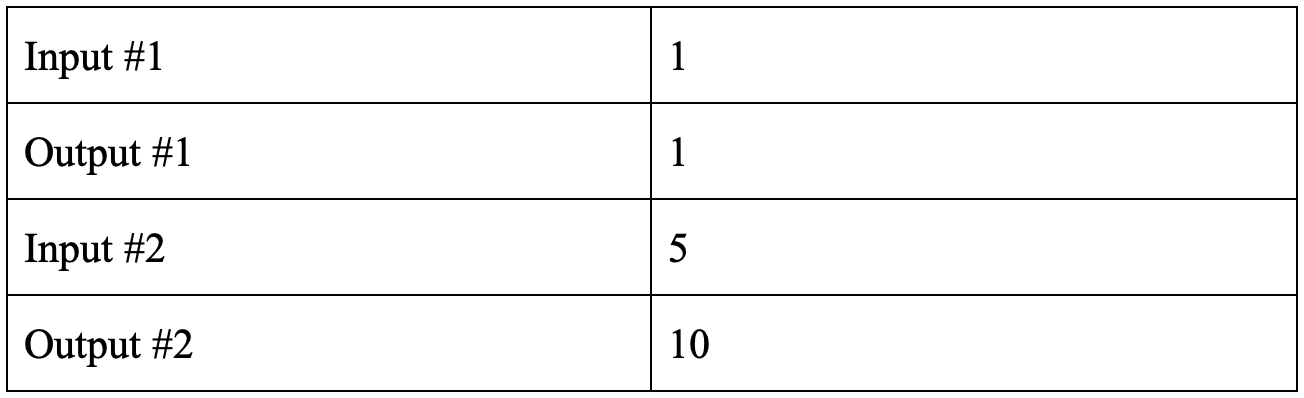
\includegraphics[width=0.80\textwidth]{q1_iodata.png}
    \end{figure}

\vspace{5pt}

\paragraph{实验环境}
\begin{itemize}
    \item 程序设计语言:C++
    \item 编程环境:
    \begin{itemize}
        \item 编辑器:Visual Studio Code (1.67.0)
        \item 编译器:g++ (GCC) 11.2.0
        \item 操作系统:ArchLinux 5.17.5-zen1-1-zen (64-bit)
    \end{itemize}
\end{itemize}

\vspace{5pt}

\paragraph{解答} 时间复杂度:$O(n!)$

源码:
\inputminted[bgcolor=codebg,frame=lines,autogobble,linenos=true,breaklines]{cpp}{src/a.cpp}

\vspace{5pt}

\paragraph{实验结果}
(可附上截图)

\newpage

\subsection*{题目2:求最大团}
\paragraph{题目内容}
\subparagraph{题目描述}
\begin{itemize}
    \item 给定一个图G(V, E),一个团表示一个子图g(v,e),满足:对所有顶点对$v1, v2 \in v$,存在一条边 (v1, v2) $ \in e$。最大团是所有团中拥有最多顶点数的那个团。
\end{itemize}

\subparagraph{输入格式}
    \begin{itemize}
        \item 第一行输入一个整数n,表示顶点数量。
        \item 紧接着n行,每一行有n个0或1的值,表示在顶点i(行号)和j(列号)之间是否存在一条边。
    \end{itemize}

\subparagraph{输出格式}
    \begin{itemize}
        \item 一个整数,表示求得的最大团中顶点数量。
    \end{itemize}
    
\subparagraph{输入输出样例}
如下表
    \begin{figure}[h]
        \centering
        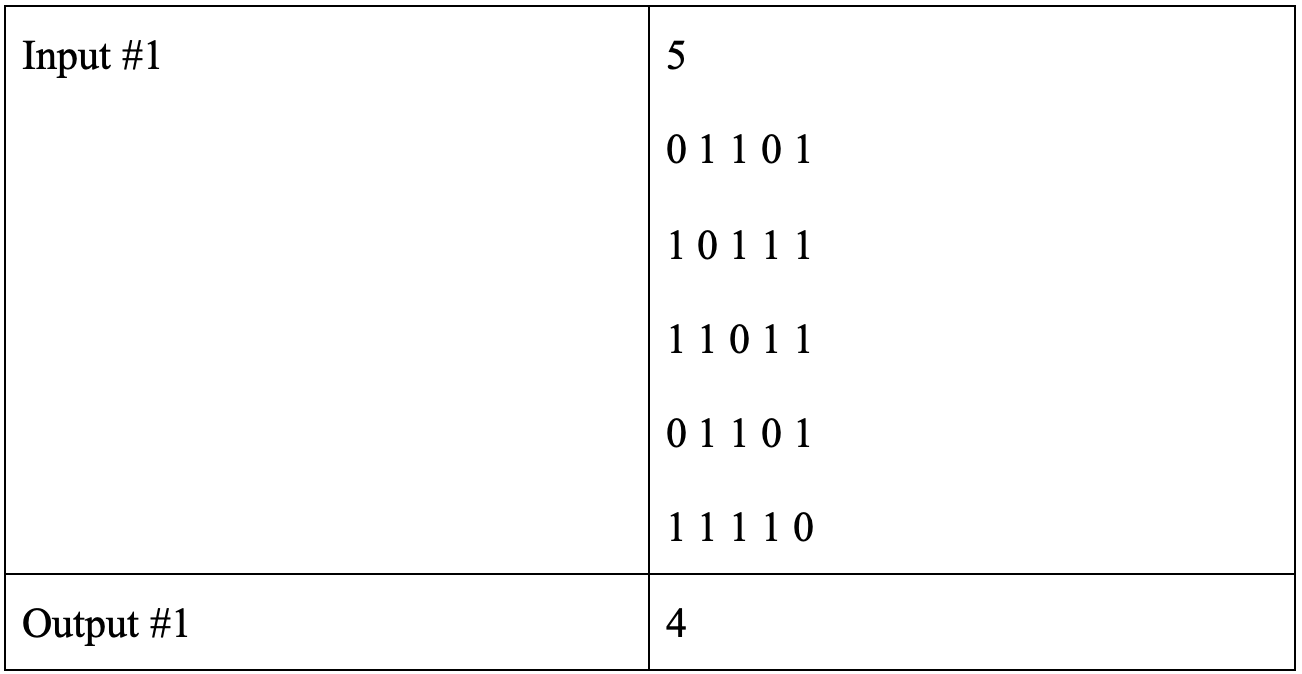
\includegraphics[width=0.80\textwidth]{q2_iodata.png}
    \end{figure}


\vspace{5pt}

\paragraph{实验环境}
\begin{itemize}
    \item 程序设计语言:C++
    \item 编程环境:
    \begin{itemize}
        \item 编辑器:Visual Studio Code (1.67.0)
        \item 编译器:g++ (GCC) 11.2.0
        \item 操作系统:ArchLinux 5.17.5-zen1-1-zen (64-bit)
    \end{itemize}
\end{itemize}

\vspace{5pt}

\paragraph{解答} 时间复杂度:$O(n^2)$

源码:
\inputminted[bgcolor=codebg,frame=lines,autogobble,linenos=true,breaklines]{cpp}{src/b.cpp}

\vspace{5pt}

\paragraph{实验结果}
(可附上截图)

\newpage

\subsection*{题目3:密码破译}
\paragraph{题目内容}
\subparagraph{题目描述}

\begin{itemize}
    \item 假设你是一名密码破译员,你收到一条包含三个间谍代号的电报。已知该密码的编码范围是0到127,超过127则视为无效编码(每个间谍代号的编码位于0到127之间,且不能含有前导0,即“04”是无效编码,“4”是有效编码),请问三个间谍成员可能有哪些组合情况(三个间谍代号各不相同)?

\end{itemize}

\subparagraph{输入格式}
    \begin{itemize}
        \item 第一行输入电报长度 n;
        \item 第二行输入电报(一串仅包含数字的字符串)。

    \end{itemize}

\subparagraph{输出格式}
    \begin{itemize}
        \item 输出所有可能的组合情况,具体格式见样例。
    \end{itemize}
    

\subparagraph{输入输出样例}
如下表
    \begin{figure}[h]
        \centering
        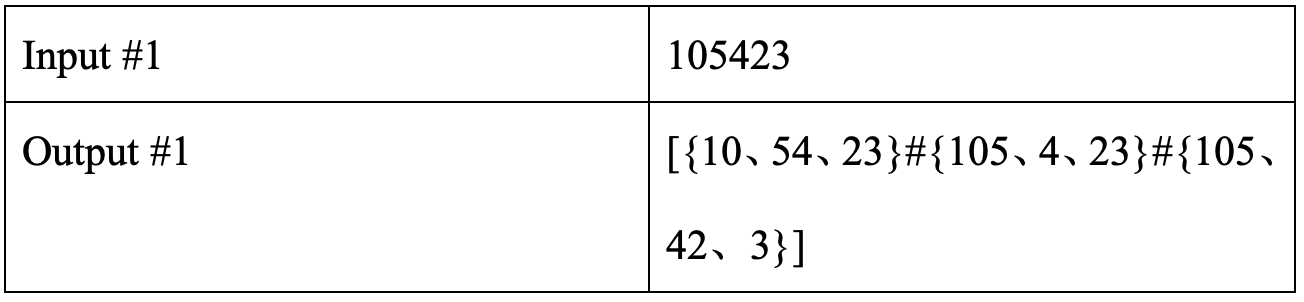
\includegraphics[width=0.80\textwidth]{q3_iodata.png}
    \end{figure}

\vspace{5pt}

\paragraph{实验环境}
\begin{itemize}
    \item 程序设计语言:C++
    \item 编程环境:
    \begin{itemize}
        \item 编辑器:Visual Studio Code (1.67.0)
        \item 编译器:g++ (GCC) 11.2.0
        \item 操作系统:ArchLinux 5.17.5-zen1-1-zen (64-bit)
    \end{itemize}
\end{itemize}

\vspace{5pt}

\paragraph{解答}

源码:
\inputminted[bgcolor=codebg,frame=lines,autogobble,linenos=true,breaklines]{cpp}{src/c.cpp}

\vspace{5pt}

\paragraph{实验结果}
(可附上截图)

\newpage

\section*{三、心得体会}
    可根据“实验思考”部分作答,也可以根据个人具体体会作答。自己算法的创新点可在此处进行介绍,酌情加分。

\end{document} 
